% Source for the figure of SuffixAutomaton (sec. 15.5): the automaton of
% abcb (above) and the one after extend(c), of abcbc (below), each state
% with its number and, under it, its len; the new state 6 and the clone 7
% of the state 3, and the transitions that extend() redirects to it, are
% shaded. Build: make figures (in ../build).
\documentclass[border=4pt]{standalone}
\usepackage[T1]{fontenc}
\usepackage{newpxtext,newpxmath}
\usepackage[varqu,varl,scaled=0.95]{zi4}
\usepackage{tikz}
% tikz-ads.tex: the TikZ styles shared by the figures of the memory of the
% manual, \input by each standalone figure: a cell of a vector (cell), the
% cell that an operation touches (touched), a free cell (free), a node of a
% linked structure (node), the labels of indices (index) and of variables
% (var), a pointer (ptr), and \cells and \indices to draw a row of cells.
\usetikzlibrary{arrows.meta,positioning,calc,fit,shapes.multipart}
\definecolor{adsTouched}{RGB}{214,196,236}
\definecolor{adsFree}{RGB}{236,236,236}
\tikzset{
  ads/.style={>={Stealth[length=2mm]},font=\small,
              every node/.append style={inner sep=0pt}},
  cell/.style={draw,minimum width=7mm,minimum height=7mm,
               font=\small\ttfamily,outer sep=0pt},
  touched/.style={cell,fill=adsTouched},
  free/.style={cell,fill=adsFree,text=black!45},
  node/.style={draw,rounded corners=1pt,minimum width=8mm,
               minimum height=6mm,font=\small\ttfamily},
  index/.style={font=\scriptsize\ttfamily,text=black!60},
  var/.style={font=\small\itshape},
  ptr/.style={->,thick}
}
% \cells{name}{x,y}{list}: a row of cells, the first at (x,y), named
% name-0, name-1, ...; each item is text/style, the style one of cell,
% touched and free (e.g., {a/cell,e/touched,/free})
\newcommand{\cells}[3]{%
  \foreach \v/\s [count=\i from 0] in {#3}
    \node[\s] (#1-\i) at ($(#2)+(\i*7mm,0)$) {\v};}
% \indices{name}{n}: the indices 0 .. n-1 under the cells of name
\newcommand{\indices}[2]{%
  \foreach \i in {0,...,\numexpr#2-1\relax}
    \node[index,below=1.2mm of #1-\i] {\i};}

\tikzset{
  st/.style={circle,draw,minimum size=6mm,font=\small},
  nw/.style={st,fill=adsTouched},
  ln/.style={font=\scriptsize,text=black!60},
  lab/.style={font=\small\ttfamily,fill=white,inner sep=1pt},
  tr/.style={->,thick},
  rd/.style={->,thick,draw=black!70}
}
\begin{document}
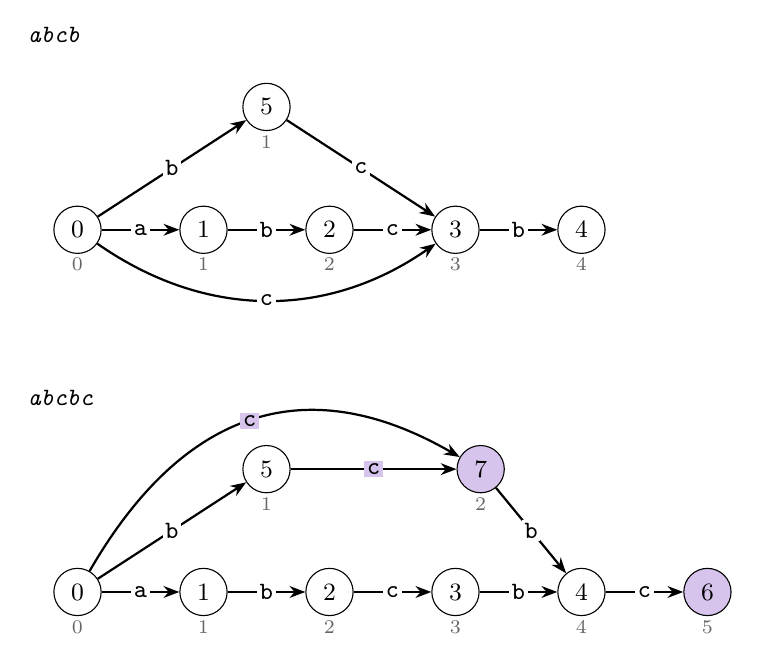
\begin{tikzpicture}[ads,x=16mm,y=13mm]
  % before: abcb
  \node[var,anchor=west] at (-0.4,1.9) {\texttt{abcb}};
  \foreach \v/\x/\y/\l in {0/0/0/0,1/1/0/1,2/2/0/2,3/3/0/3,4/4/0/4,5/1.5/1.2/1}
    { \node[st] (a\v) at (\x,\y) {\v};
      \node[ln,below=0.5mm of a\v] {\l}; }
  \draw[tr] (a0) -- node[lab] {a} (a1);
  \draw[tr] (a1) -- node[lab] {b} (a2);
  \draw[tr] (a2) -- node[lab] {c} (a3);
  \draw[tr] (a3) -- node[lab] {b} (a4);
  \draw[tr] (a0) -- node[lab] {b} (a5);
  \draw[tr] (a5) -- node[lab] {c} (a3);
  \draw[tr] (a0) to[out=-35,in=-145] node[lab] {c} (a3);
  % after extend(c): abcbc
  \begin{scope}[yshift=-46mm]
  \node[var,anchor=west] at (-0.4,1.9) {\texttt{abcbc}};
  \foreach \v/\x/\y/\l/\s in {0/0/0/0/st,1/1/0/1/st,2/2/0/2/st,3/3/0/3/st,
      4/4/0/4/st,6/5/0/5/nw,5/1.5/1.2/1/st,7/3.2/1.2/2/nw}
    { \node[\s] (b\v) at (\x,\y) {\v};
      \node[ln,below=0.5mm of b\v] {\l}; }
  \draw[tr] (b0) -- node[lab] {a} (b1);
  \draw[tr] (b1) -- node[lab] {b} (b2);
  \draw[tr] (b2) -- node[lab] {c} (b3);
  \draw[tr] (b3) -- node[lab] {b} (b4);
  \draw[tr] (b4) -- node[lab] {c} (b6);
  \draw[tr] (b0) -- node[lab] {b} (b5);
  \draw[tr] (b5) -- node[lab,fill=adsTouched] {c} (b7);
  \draw[tr] (b7) -- node[lab] {b} (b4);
  \draw[tr] (b0) to[out=60,in=150,looseness=1.2] node[lab,fill=adsTouched] {c} (b7);
  \end{scope}
\end{tikzpicture}
\end{document}
